\begin{figure}[H]
    \centering
    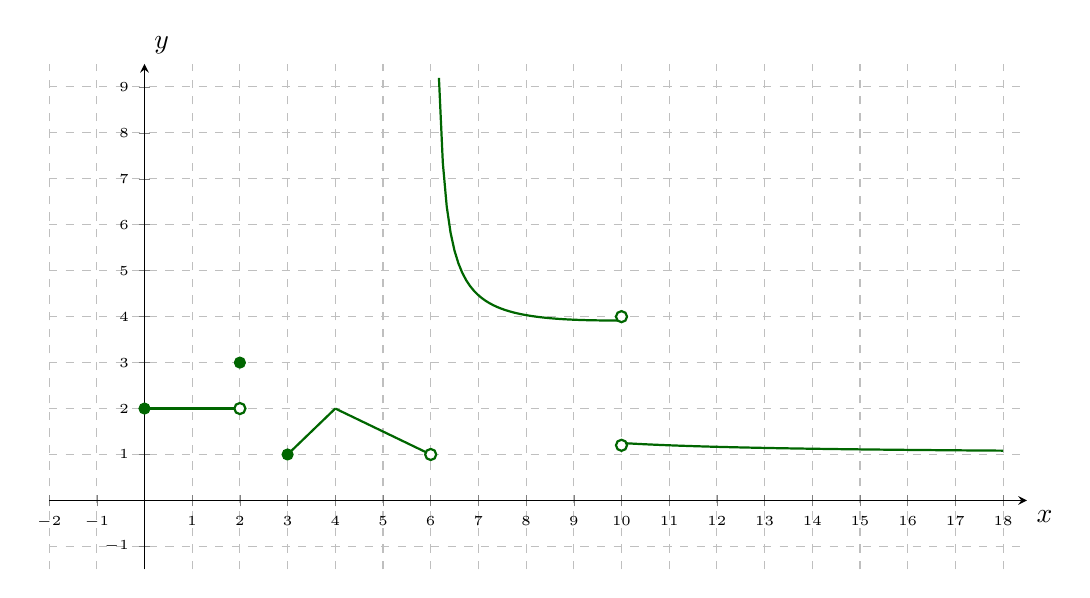
\begin{tikzpicture}
        \begin{axis}[
            axis lines=middle,
            xlabel=$x$,
            ylabel=$y$,
            xmin=-2, xmax=18.5,
            ymin=-1.5, ymax=9.5,
            grid=major,
            grid style={dashed, gray!50},
            xtick={-2,-1,0,1,...,18},
            ytick={-1,0,1,...,9},
            width=14cm,
            height=8cm,
            tick label style={font=\tiny},
            xlabel style={anchor=north west},
            ylabel style={anchor=south west},
            no markers % Tắt các marker tự động
        ]
            % Định nghĩa màu sắc cho đồ thị
            \colorlet{mygreen}{green!40!black}

            % --- Vẽ các đoạn của hàm số ---
            
            % 1. Đoạn ngang y=2, từ x=0 đến x=2
            \addplot[mygreen, thick, domain=0:2] {2};

            % 2. Hình chữ V, từ (3,1) đến (4,2) rồi đến (6,1)
            \addplot[mygreen, thick, domain=3:4] {x-2};
            \addplot[mygreen, thick, domain=4:6] {-0.5*x + 4};

            % 3. Nhánh Hyperbola với tiệm cận đứng x=6
            % Vẽ phần gần tiệm cận, giới hạn chiều cao để không bị vỡ hình
            \addplot[mygreen, thick, domain=6.01:10, samples=50, restrict y to domain=-1.5:10.5] {1/(x-6) + 1/15*x + 3};
            % Vẽ phần còn lại của nhánh hyperbola
            \addplot[mygreen, thick, domain=10:18, samples=50] {1/(x-6) + 1};

            % --- Đánh dấu các điểm đặc biệt ---
            
            % Các điểm được tô đầy (included)
            \addplot[only marks, mark=*, mygreen, mark size=2pt, fill=mygreen] coordinates {
                (0,2)   % Điểm bắt đầu của đoạn ngang
                (2,3)   % Điểm riêng lẻ ở trên
                (3,1)   % Điểm bắt đầu của hình chữ V
            };

            % Các điểm rỗng (excluded)
            \addplot[only marks, mark=o, mygreen, mark size=2pt, draw=mygreen, fill=white, thick] coordinates {
                (2,2)   % Điểm kết thúc của đoạn ngang
                (6,1)   % Điểm kết thúc của hình chữ V
                (10,4)   % Điểm bị loại trừ trên nhánh hyperbola
                (10,1.2) % Điểm bị loại trừ trên nhánh hyperbola
            };

        \end{axis}
    \end{tikzpicture}
    \caption{Hình 3.1.4}
    \label{fig:complex_piecewise_graph}
\end{figure}
